\documentclass[12pt]{article}
%%---------------------------------------------------------------------
% packages
% geometry
\usepackage{geometry}
% font
\usepackage{fontspec}
\defaultfontfeatures{Mapping=tex-text}  %%如果没有它,会有一些 tex 特殊字符无法正常使用,比如连字符。
\usepackage{xunicode,xltxtra}
\usepackage[BoldFont,SlantFont,CJKnumber,CJKchecksingle]{xeCJK}  % \CJKnumber{12345}: 一万二千三百四十五
\usepackage{CJKfntef}  %%实现对汉字加点、下划线等。
\usepackage{pifont}  % \ding{}
% math
\usepackage{amsmath,amsfonts,amssymb}
% color
\usepackage{color}
\usepackage{xcolor}
\definecolor{EYE}{RGB}{199,237,204}
\definecolor{FLY}{RGB}{128,0,128}
\definecolor{ZHY}{RGB}{139,0,255}
% graphics
\usepackage[americaninductors,europeanresistors]{circuitikz}
\usepackage{tikz}
\usetikzlibrary{positioning,arrows,shadows,shapes,calc,mindmap,trees,backgrounds}  % placements=positioning
\usepackage{graphicx}  % \includegraphics[]{}
\usepackage{subfigure}  %%图形或表格并排排列
% table
\usepackage{colortbl,dcolumn}  %% 彩色表格
\usepackage{multirow}
\usepackage{multicol}
\usepackage{booktabs}
% code
\usepackage{fancyvrb}
\usepackage{listings}
% title
\usepackage{titlesec}
% head/foot
\usepackage{fancyhdr}
% ref
\usepackage{hyperref} %生成可链接目录
% pagecolor
\usepackage[pagecolor={EYE}]{pagecolor}
% tightly-packed lists
\usepackage{mdwlist}
\usepackage{verbatim}%comment命令的注释包
\usepackage{styles/iplouccfg}
\usepackage{styles/zhfontcfg}
\usepackage{styles/iplouclistings}
%%---------------------------------------------------------------------
% settings
% geometry
\geometry{left=2cm,right=1cm,top=2cm,bottom=2cm}  %设置 上、左、下、右 页边距
\linespread{1.5} %行间距
% font
\setCJKmainfont{Adobe Kaiti Std}
%\setmainfont[BoldFont=Adobe Garamond Pro Bold]{Apple Garamond}  % 英文字体
%\setmainfont[BoldFont=Adobe Garamond Pro Bold,SmallCapsFont=Apple Garamond,SmallCapsFeatures={Scale=0.7}]{Apple Garamond}  %%苹果字体没有SmallCaps
\setCJKmonofont{Adobe Fangsong Std}
% graphics
\graphicspath{{figures/}}
\tikzset{
    % Define standard arrow tip
    >=stealth',
    % Define style for boxes
    punkt/.style={
           rectangle,
           rounded corners,
           draw=black, very thick,
           text width=6.5em,
           minimum height=2em,
           text centered},
    % Define arrow style
    pil/.style={
           ->,
           thick,
           shorten <=2pt,
           shorten >=2pt,},
    % Define style for FlyZhyBall
    FlyZhyBall/.style={
      circle,
      minimum size=6mm,
      inner sep=0.5pt,
      ball color=red!50!blue,
      text=white,},
    % Define style for FlyZhyRectangle
    FlyZhyRectangle/.style={
      rectangle,
      rounded corners,
      minimum size=6mm,
      ball color=red!50!blue,
      text=white,},
    % Define style for zhyfly
    zhyfly/.style={
      rectangle,
      rounded corners,
      minimum size=6mm,
      ball color=red!25!blue,
      text=white,},
    % Define style for new rectangle
    nrectangle/.style={
      rectangle,
      draw=#1!50,
      fill=#1!20,
      minimum size=5mm,
      inner sep=0.1pt,}
}
\ctikzset{
  bipoles/length=.8cm
}
% code
\lstnewenvironment{VHDLcode}[1][]{%
  \lstset{
    basicstyle=\footnotesize\ttfamily\color{black},%
    columns=flexible,%
    framexleftmargin=.7mm,frame=shadowbox,%
    rulesepcolor=\color{blue},%
%    frame=single,%
    backgroundcolor=\color{yellow!20},%
    xleftmargin=1.2\fboxsep,%
    xrightmargin=.7\fboxsep,%
    numbers=left,numberstyle=\tiny\color{blue},%
    numberblanklines=false,numbersep=7pt,%
    language=VHDL%
    }\lstset{#1}}{}
\lstnewenvironment{VHDLmiddle}[1][]{%
  \lstset{
    basicstyle=\scriptsize\ttfamily\color{black},%
    columns=flexible,%
    framexleftmargin=.7mm,frame=shadowbox,%
    rulesepcolor=\color{blue},%
%    frame=single,%
    backgroundcolor=\color{yellow!20},%
    xleftmargin=1.2\fboxsep,%
    xrightmargin=.7\fboxsep,%
    numbers=left,numberstyle=\tiny\color{blue},%
    numberblanklines=false,numbersep=7pt,%
    language=VHDL%
    }\lstset{#1}}{}
\lstnewenvironment{VHDLsmall}[1][]{%
  \lstset{
    basicstyle=\tiny\ttfamily\color{black},%
    columns=flexible,%
    framexleftmargin=.7mm,frame=shadowbox,%
    rulesepcolor=\color{blue},%
%    frame=single,%
    backgroundcolor=\color{yellow!20},%
    xleftmargin=1.2\fboxsep,%
    xrightmargin=.7\fboxsep,%
    numbers=left,numberstyle=\tiny\color{blue},%
    numberblanklines=false,numbersep=7pt,%
    language=VHDL%
    }\lstset{#1}}{}
% pdf
\hypersetup{pdfauthor={Haiyong Zheng},%
            pdftitle={Title},%
            CJKbookmarks=true,%
            bookmarksnumbered=true,%
            bookmarksopen=false,%
            plainpages=false,%
            colorlinks=true,%
            citecolor=green,%
            filecolor=magenta,%
            linkcolor=cyan,%red(default)
            urlcolor=cyan}
% section
%http://tex.stackexchange.com/questions/34288/how-to-place-a-shaded-box-around-a-section-label-and-name
\newcommand\titlebar{%
\tikz[baseline,trim left=3.1cm,trim right=3cm] {
    \fill [cyan!25] (2.5cm,-1ex) rectangle (\textwidth+3.1cm,2.5ex);
    \node [
        fill=cyan!60!white,
        anchor= base east,
        rounded rectangle,
        minimum height=3.5ex] at (3cm,0) {
        \textbf{\thesection.}
    };
}%
}
\titleformat{\section}{\Large\bf\color{blue}}{\titlebar}{0.1cm}{}
% head/foot
\setlength{\headheight}{15pt}
\pagestyle{fancy}
\fancyhf{}
\numberwithin{equation}{section}%%公式与章节关联
%\lhead{\color{black!50!green}2014年秋季学期}
\chead{\color{black!50!green}Machine Learning Note}
%\rhead{\color{black!50!green}通信电子电路}
\lfoot{\color{blue!50!green}常琳}
%\cfoot{\color{blue!50!green}\href{http://vision.ouc.edu.cn/~zhenghaiyong}{CVBIOUC}}
\rfoot{\color{blue!50!green}$\cdot$\ \thepage\ $\cdot$}
\renewcommand{\headrulewidth}{0.4pt}
\renewcommand{\footrulewidth}{0.4pt}

%%---------------------------------------------------------------------
\begin{document}
%%---------------------------------------------------------------------
%%---------------------------------------------------------------------
% \titlepage
\title{\vspace{-2em}Machine Learning Note\vspace{-0.7em}}
\author{}
\date{}
%%---------------------------------------------------------------------
\maketitle\thispagestyle{fancy}
%%---------------------------------------------------------------------
\maketitle
\tableofcontents 
%---------------------------------------------------------------------

\linespread{1.5} %行间距

%=======================================================================

\section{模型评估与选择}

\subsection{经验误差与过拟合}

学习器在训练集上的误差称为``训练误差"或``经验误差"(empirical error),在新样本上的误差称为``泛化误差"(generalization error).

``过拟合":训练样本学的太好,泛化性能下降      /quad 是机器学习的关键障碍,无法彻底避免

``欠拟合":是指对训练样本的一般性质尚未学好

\subsection{评估方法}

现实中要考虑时间开销,存储开销,可解释性等方面因素,这里只考虑泛化误差.

\subsubsection{留出法}

直接将数据集D划分为两个互斥的集合,训练集S和测试集T.训练/测试集的划分要尽量保持数据分布的一致性.

单次使用留出法得到的估计结果不够稳定可靠,一般采用多次随机划分,重复试验取平均值作为评估结果.

\subsubsection{交叉验证法}

先将数据集D划分成k个(k折)大小相似的互斥子集,每个子集都尽可能保持数据分布的一致性,即从D中通过分层采样得到. 然后每次用k-1个子集的并集作为训练集, 余下子集作为测试集,进行k次训练和测试,最终返回的是k个测试结果的均值.

为减小因样本划分不同而引入的差别,k折要随机用不同的划分重复p次,最终评估结果是p次k折交叉验证结果的均值.

假定D包含m个样本,若令k=m, 得到特例: 留一法 (Leave-One-Out, LOO)









%%----------------------------------------------------------------------------------------------------------------------------------------------------------------------------------------------------
\section{支持向量机}

\subsection{间隔与支持向量}

机器学习中可以用于分类或者回归问题. 这里主要是分类.

超平面: 二维空间的超平面是一条直线,三维空间的超平面是一个平面,而N维空间的超平面则是N-1维的仿射空间.

超平面性质: 将空间分成两部分,一部分大于0,一部分小于0.

凸二次规划问题: \url{https://zhidao.baidu.com/question/281998847.html}

样本空间中划分超平面:

\begin{equation}
\boldsymbol{\omega}^{T}\boldsymbol{x}+b=0
\end{equation}

\boldmath$\omega$  \unboldmath = $\{\omega_{1};\omega_{2};\ldots \omega_{d}\}$ 为法向量,决定超平面的方向; $b$ 为位移项,决定超平面与原点之间的距离.

样本空间任一点\boldmath$x$到超平面 \boldmath($\omega$, \unboldmath$b$) 的距离:

\begin{equation}
r=\dfrac{\mid \boldsymbol{\omega}^{T}\boldsymbol{x}+b \mid}{\parallel \boldsymbol{\omega} \parallel}
\end{equation}

设超平面 \boldmath($\omega$, \unboldmath$b$)能将训练样本正确分类,即对于超平面 \boldmath($x_{i}$, \unboldmath$y_{i}$) $\in D$,若$y_{i}=+1$, 则有
$ \boldsymbol{\omega}^{T}\boldsymbol{x}+b>0$; 若 $y_{i}=-1$, $ \boldsymbol{\omega}^{T}\boldsymbol{x}+b<0$. 另

\begin{equation}
\label{6-3}
 \left\{ \begin{array}{ll}
 \boldsymbol{\omega}^{T}\boldsymbol{x}_{i}+b \geqslant +1 & \textrm{ $y_{i}=+1$}\\
\boldsymbol{\omega}^{T}\boldsymbol{x}_{i}+b \leqslant -1  &  \textrm{ $y_{i}=-1$}\\
\end{array} \right.
\end{equation}

\textcolor[rgb]{0.2,0.3,0.6}{注: 若存在超平面 $(\boldsymbol{\omega}', b')$ 能将训练样本正确分类, 则总存在缩放变换 $\zeta \boldsymbol{\omega} \longmapsto \boldsymbol{\omega}'$ 和 $\zeta b \longmapsto b'$ 使式\ref{6-3}成立.}

如图\ref{6-2}, 距离超平面最近的几个样本点使式\ref{6-3}的等号成立,每个样本点对应一个特征向量, 他们被称为``支持向量", 两个异类支持向量到超平面的距离和:

\begin{equation}
\gamma=\frac{2}{\parallel \boldsymbol{\omega} \parallel}
\end{equation}
称为``间隔"(margin)(这里的"间隔"指几何间隔).
\begin{figure}
\centering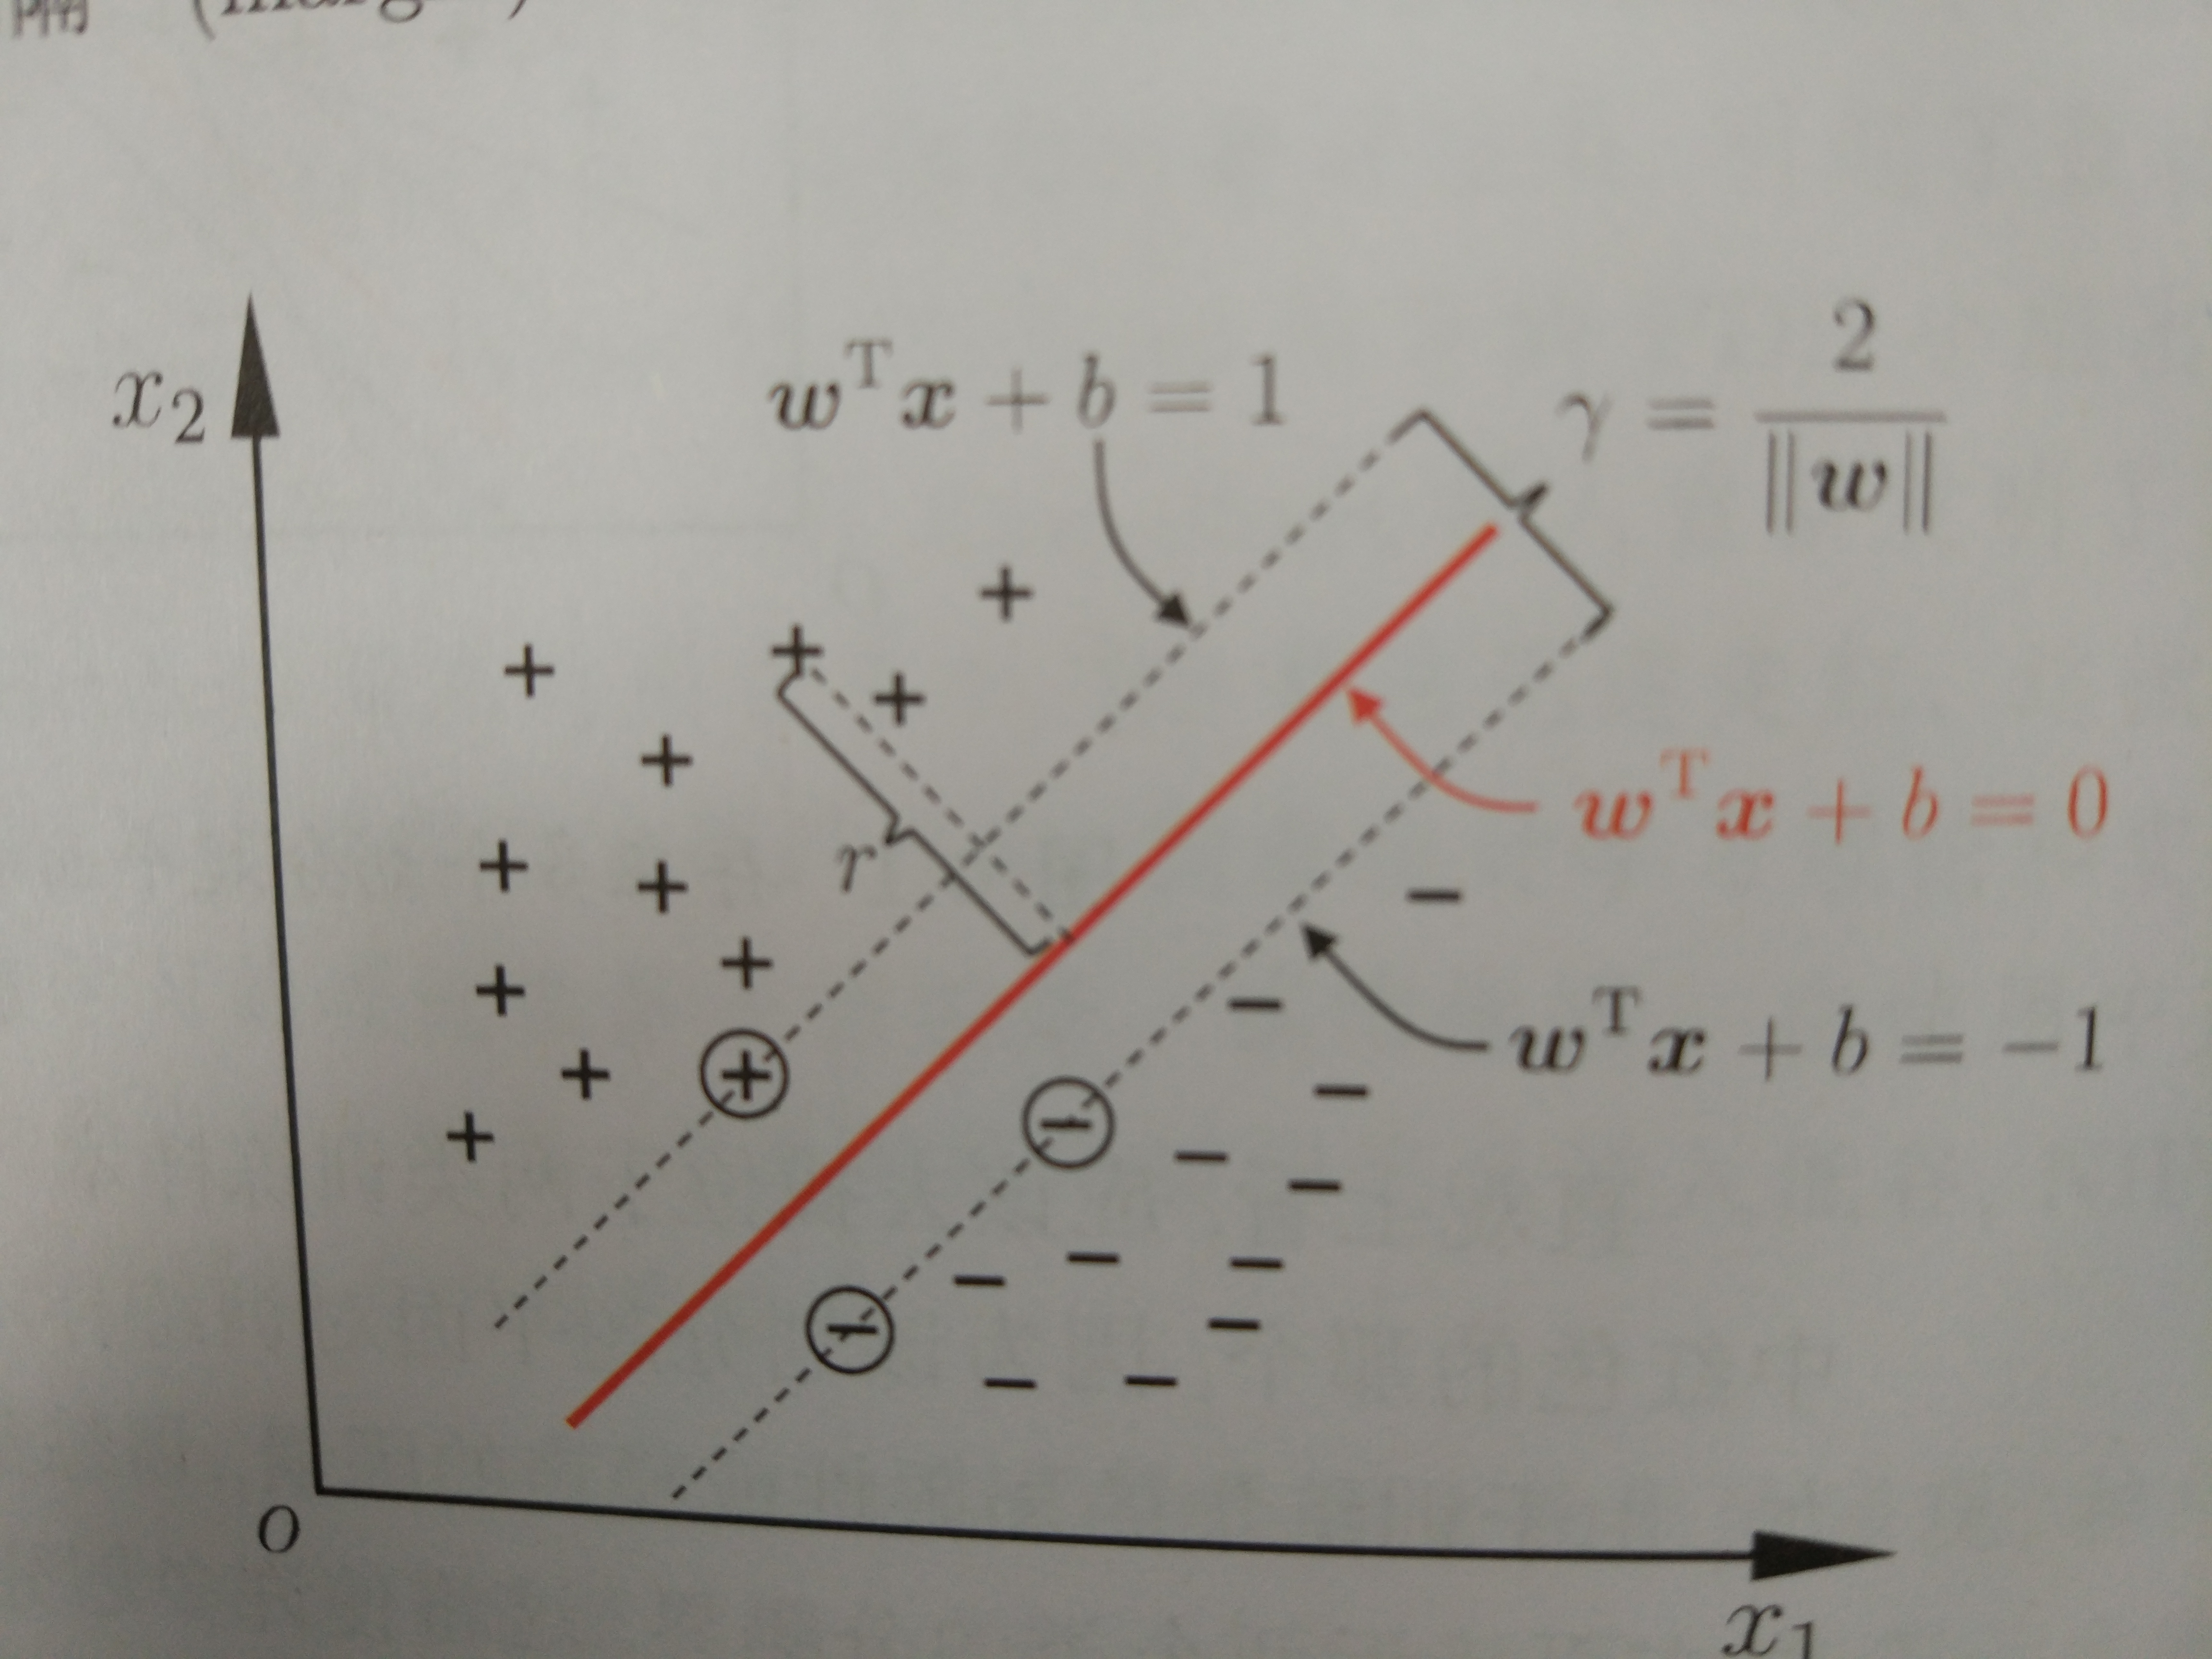
\includegraphics[width=5in]{6-2.jpg}
\caption{支持向量与间隔}
\label{6-2}
\end{figure}

欲找到具有``最大间隔"(maximum margin)的划分超平面,即



\begin{equation}
\begin{split}        %换行 
 {\underset{\boldsymbol{\omega},b}{max}} \quad \frac{2}{\parallel \boldsymbol{\omega} \parallel}  \\
 s.t. \quad y_{i}(\boldsymbol{\omega}^{T}\boldsymbol{x}_{i}+b) \geqslant 1, \quad i= 1,2, \ldots ,m.
\end{split}
\label{6-5}
\end{equation}

$b$通过约束隐式地影响$\boldsymbol{\omega}$,所以间隔与$b$和$\boldsymbol{\omega}$都有关.

式\ref{6-5}可以重写为:

\begin{equation}
\begin{split}        %换行 
 {\underset{\boldsymbol{\omega},b}{min}} \quad \frac{\parallel \boldsymbol{\omega} \parallel^{2}}{2} \\
 s.t. \quad y_{i}(\boldsymbol{\omega}^{T}\boldsymbol{x}_{i}+b) \geqslant 1, \quad i= 1,2, \ldots ,m.
\end{split}
\label{6-6}
\end{equation}

即支持向量机(SVM)的基本型.

\subsection{对偶问题}

希望通过解式\ref{6-6}得到大间隔划分超平面对应的模型

\begin{equation}
f(x)=\boldsymbol{\omega}^{T}\boldsymbol{x}+b
\label{6-7}
\end{equation}

对式\ref{6-6}使用拉格朗日乘子法可得到其``对偶问题"(线性规划有一个有趣的特性,就是任何一个求极大的问题都有一个与其匹配的求极小的线性规划问题). 对偶问题可以更高效地求解模型参数$\boldsymbol{\omega}, b$, 对\ref{6-6}每条约束添加拉格朗日乘子$\alpha_{i} \geqslant 0$,拉格朗日函数可写为

\begin{equation}
L(\boldsymbol{\omega},b,\boldsymbol{\alpha})=\frac{\parallel \boldsymbol{\omega} \parallel^{2}}{2}+\sum_{i=1}^{m}\alpha_{i}(1-y_{i}(\boldsymbol{\omega}^{T}\boldsymbol{x}_{i}+b))
\label{6-8}
\end{equation}

$\boldsymbol{\alpha}=(\alpha_{1};\alpha_{2};\ldots;\alpha_{m})$, 令$L(\boldsymbol{\omega},b,\boldsymbol{\alpha})$对$\boldsymbol{\omega}$和$b$的偏导为0得

\begin{equation}
\boldsymbol{\omega}=\sum_{i=1}^{m}\alpha_{i}y_{i}\boldsymbol{x}_{i}
\label{6-9}
\end{equation}

\begin{equation}
0=\sum_{i=1}^{m}\alpha_{i}y_{i}
\label{6-10}
\end{equation}

\ref{6-9}代入\ref{6-8},考虑\ref{6-10}的约束,就可得到\ref{6-6}的对偶问题

\begin{equation}
\begin{split} 
{\underset{\boldsymbol{\alpha}}{max}} \quad  \sum_{i=1}^{m}\alpha_{i}-\dfrac{1}{2}\sum_{i=1}^{m}\sum_{j=1}^{m}\alpha_{i}\alpha_{j}y_{i}y_{j}{\boldsymbol{x}}_{i}^{T}{\boldsymbol{x}}_{j}  \\
s.t. \quad \sum_{i=1}^{m}\alpha_{i}y_{i} = 0,  \\
\alpha_{i} \geqslant 0, \quad i=1,2, \ldots, m 
\end{split}
\label{6-11}
\end{equation}

(这里的对偶问题式子里没出现b, 貌似因为式\ref{6-6}里显示间隔只和 $\boldsymbol{\omega}$ 有关,所以这里把b 那项忽略了)

解出$\boldsymbol{\alpha}$, 求出$\boldsymbol{\omega}$与$b$即可得到模型

\begin{equation}
f(\boldsymbol{x})=\boldsymbol{\omega}^{T}\boldsymbol{x}+b=\sum_{i=1}^{m}\alpha_{i}y_{i}{\boldsymbol{x}}_{i}^{T}{\boldsymbol{x}}+b
\label{6-12}
\end{equation}

因式\ref{6-6}中有不等式约束,上述过程需满足KKT(Karush-Kuhn-Tucker)条件, 即要求

\begin{equation}
 \left\{ \begin{array}{ll}
\alpha_{i} \geqslant 0;\\
 y_{i}f(\boldsymbol{x}_{i})-1\geqslant 0; \\
 \alpha_{i}(y_{i}f(\boldsymbol{x}_{i})-1) = 0.
\end{array} \right.
\end{equation}

(关于KKT条件和拉格朗日乘子的详细解释: \url{http://blog.csdn.net/xianlingmao/article/details/7919597})

于是,对于任意训练样本$(\boldsymbol{x}_{i},y_{i})$,总有$\alpha_{i}=0$或$y_{i}f(\boldsymbol{x}_{i}) =1$. 若$\alpha_{i}=0$, 则该样本不会在式\ref{6-12}中出现,也就不会对$f(\boldsymbol{x})$产生影响;若$\alpha_{i} > 0$, 则必有$y_{i}f(\boldsymbol{x}_{i})=1$,所对应的样本点位于最大间隔边界上,是一个支持向量.因此,{\color{red}{训练完成后,大部分的训练样本都不需要保留,最终模型仅与支持向量有关.}}

此外,{\color{blue}求解式\ref{6-11},可以用SMO算法.}(见svm程序部分)

Sequential Minimal Optimization (SMO) 基本思路: 先固定$\alpha_{i}$以外的所有参数,然后求$\alpha_{i}$上的极值. 由于存在约束 $ \sum_{i=1}^{m}\alpha_{i}y_{i} = 0$, 若固定$\alpha_{i}$以外的其他变量, $\alpha_{i}$可由其他变量导出.

在参数初始化后, SMO不断执行如下两个步骤直至收敛:

\begin{itemize}
\item 选取一对需更新的变量$\alpha_{i}$和$\alpha_{j}$ (为了满足约束条件$ \sum_{i=1}^{m}\alpha_{i}y_{i} = 0$,所以每次需更新一对)

\item 固定$\alpha_{i}$和$\alpha_{j}$ , 求解式\ref{6-11}获得更新后的$\alpha_{i}$和$\alpha_{j}$ .
\end{itemize}

SMO的变量选取方式: 使选取的两变量所对应样本之间的间隔最大.

偏移项$b$的确定: 对任意支持向量$(\boldsymbol{x}_{s},y_{s})$都有$y_{s}f(\boldsymbol{x}_{s})=1$, 即

\begin{equation}
y_{s}(\sum_{i \in S}\alpha_{i}y_{i}\boldsymbol{x}_{i}^{T}\boldsymbol{x}_{s}+b)=1
\label{6-17}
\end{equation}

$S=\{i\mid \alpha_{i} > 0, i=1, 2, \ldots, m\}$为所有支持向量的下标集. 理论上, 可选任意支持向量并通过式\ref{6-17}获得$b$, 实际中:

\begin{equation}
b=\frac{1}{\mid S\mid}\sum_{s\in S}(y_{s}-\sum_{i \in S}\alpha_{i}y_{i}\boldsymbol{x}_{i}^{T}\boldsymbol{x}_{s})
\end{equation}



\subsection{核函数}

不是所有的原始样本空间都存在能正确划分两类样本的超平面.可将样本从\textbf{原始空间}映射到一个\textbf{更高维的特征空间}. 如果原始空间是有限维,那么一定存在一个高维特征空间使样本可分.

令$\Phi(\boldsymbol{x})$表示将$\boldsymbol{x}$映射后的特征向量,在特征空间中划分超平面所对应的模型为

\begin{equation}
f(\boldsymbol{x})=\boldsymbol{\omega}^{T}\Phi(\boldsymbol{x})+b
\end{equation}

对偶问题什么的和之前都差不多

\begin{equation}
\begin{split} 
{\underset{\boldsymbol{\alpha}}{max}} \quad  \sum_{i=1}^{m}\alpha_{i}-\dfrac{1}{2}\sum_{i=1}^{m}\sum_{j=1}^{m}\alpha_{i}\alpha_{j}y_{i}y_{j}\Phi(\boldsymbol{x}_{i})^{T}\Phi(\boldsymbol{x}_{j})  \\
s.t. \quad \sum_{i=1}^{m}\alpha_{i}y_{i} = 0,  \\
\alpha_{i} \geqslant 0, \quad i=1,2, \ldots, m 
\end{split}
\label{6-21}
\end{equation}

特征空间维数可能很高,直接计算$\Phi(\boldsymbol{x}_{i})^{T}\Phi(\boldsymbol{x}_{j}) $通常困难,设想一个函数:

\begin{equation}
\kappa(\boldsymbol{x}_{i},\boldsymbol{x}_{j})=<\Phi(\boldsymbol{x}_{i}),\Phi(\boldsymbol{x}_{j}) >=\Phi(\boldsymbol{x}_{i})^{T}\Phi(\boldsymbol{x}_{j}) 
\end{equation}

{\color{blue}{即$\boldsymbol{x}_{i}$和$\boldsymbol{x}_{j}$在\textbf{特征空间}的內积等于它们在\textbf{原始样本空间}中通过\textbf{``核函数"$\kappa(.,.)$}计算的结果}}. 式\ref{6-21}重写为

\begin{equation}
\begin{split} 
{\underset{\boldsymbol{\alpha}}{max}} \quad  \sum_{i=1}^{m}\alpha_{i}-\dfrac{1}{2}\sum_{i=1}^{m}\sum_{j=1}^{m}\alpha_{i}\alpha_{j}y_{i}y_{j}\kappa(\boldsymbol{x}_{i},\boldsymbol{x}_{j})  \\
s.t. \quad \sum_{i=1}^{m}\alpha_{i}y_{i} = 0,  \\
\alpha_{i} \geqslant 0, \quad i=1,2, \ldots, m 
\end{split}
\label{6-23}
\end{equation}

求解后得到

\begin{equation}
\begin{split} 
f(\boldsymbol{x})=\boldsymbol{\omega}^{T}\Phi(\boldsymbol{x})+b \\
= \sum_{i=1}^{m}\alpha_{i}y_{i}\Phi(\boldsymbol{x}_{i})^{T}\Phi(\boldsymbol{x})+b  \\
=\sum_{i=1}^{m}\alpha_{i}y_{i}\kappa(\boldsymbol{x},\boldsymbol{x}_{i})+b
\end{split} 
\label{6-24}
\end{equation}

式\ref{6-24}显示出模型最优解就可通过训练样本的核函数展开,这一展式也称``支持向量展示".

\textbf{定理6.1 (核函数)}  \quad 令$\chi$ 为输入空间,$\kappa(.,.)$是定义在$\chi \times \chi$上的对称函数,则$\kappa$是核函数当且仅当对于任意数据$D=\{\boldsymbol{x}_{1},\boldsymbol{x}_{2},\ldots,\boldsymbol{x}_{m}\}$,``核矩阵"$K$总是半正定的.
 定理6.1表明,只要一个对称函数所对应的核矩阵半正定,它就能作为核函数使用.事实上,对于一个半正定核矩阵,总能找到一个与之对应的映射$\Phi$

\textbf{常用核函数:} 

线性核, \quad $ \kappa(\boldsymbol{x}_{i},\boldsymbol{x}_{j}) =  \boldsymbol{x}_{i}^{T}\boldsymbol{x}_{j}$

多项式核, \quad $ \kappa(\boldsymbol{x}_{i},\boldsymbol{x}_{j}) =  (\boldsymbol{x}_{i}^{T}\boldsymbol{x}_{j})^{d}$

高斯核(亦称RBF核),  \quad $\kappa(\boldsymbol{x}_{i},\boldsymbol{x}_{j}) =  exp(-\frac{\Vert \boldsymbol{x}_{i} - \boldsymbol{x}_{j}\Vert^{2}}{2\sigma ^{2}}) $

拉普拉斯核,  Sigmoid核,还有函数组合的核.

\subsection{软间隔与正则化}

现实中很难确定合适的核函数使得训练样本在特征空间中线性可分,即使找到了,可分的结果也许是过拟合造成的.

缓解的一个办法是允许支持向量机在一些样本上出错.为此,引入图\ref{6.4}``软间隔"(soft margin)概念.

\begin{figure}
\centering\includegraphics[width=5in]{6-4.jpg}
\caption{软间隔}
\label{6.4}
\end{figure}

支持向量机形式是要求所有样本均满足约束\ref{6-3}, 即所有样本都必须划分正确,称``硬间隔"(hard margin).软间隔允许某些样本不满足约束(不满足约束的样本应尽可能少)

\begin{equation}
y_{i}(\boldsymbol{\omega}^{T}\boldsymbol{x}_{i}+b) \geqslant 1
\label{6-28}
\end{equation}

优化目标为

\begin{equation}
{\underset{\boldsymbol{\omega},b}{min}} \quad \dfrac{1}{2}||\omega||^{2}+C\sum_{i=1}^{m}l_{0/1}(y_{i}(\boldsymbol{\omega}^{T}\boldsymbol{x}_{i}+b)-1)
\label{6-29}
\end{equation}

(原来的是那个${\underset{\boldsymbol{\omega},b}{min}} \quad \dfrac{1}{2}||\omega||^{2}$)

$C>0$是常数, $l_{0/1}$是``$0/1$损失函数"

\begin{equation}
l_{0/1}(z)=
 \left\{ \begin{array}{ll}
1 \quad if  \quad z<0;\\
 0 \quad otherwise
\end{array} \right.
\end{equation}

当$C$为无穷大时,式\ref{6-29}迫使所有样本均满足约束\ref{6-28}(不满足的话,\ref{6-29}会无穷大),\ref{6-29}等价于\ref{6-6}; $C$取有限值时,\ref{6-29}允许一些样本不满足约束.

$l_{0/1}$非凸,非连续,数学性质不太好,使式\ref{6-29}不易直接求解(??),常用其他函数替代之,称``替代损失". 替代损失函数一般具有较好的数学性质,如通常是凸的连续函数且是$l_{0/1}$的上界(这个也算优点???!!!). 三种常用替代损失函数(图\ref{6.5}):

hinge损失: 
\begin{equation}
l_{hinge}(z) = max(0, 1 - z);
\end{equation}

指数损失(exponential loss): 	
\begin{equation}
l_{exp}(z) = exp( - z);
\end{equation}

对率损失(logistic loss): 
\begin{equation}
l_{log}(z) = log(1+exp( - z));
\end{equation}



%\begin{comment}
\begin{figure}
\centering\includegraphics[width=6in]{6-5.jpg}
\caption{三种常见的替代损失函数:hinge损失, 指数损失, 对率损失}
\label{6.5}
\end{figure}
%\end{comment}

若采用hinge损失, 式\ref{6-29}变成

\begin{equation}
{\underset{\boldsymbol{\omega},b}{min}} \quad \dfrac{1}{2}\Vert \boldsymbol{\omega}\Vert^{2}+C\sum_{i=1}^{m}max(0, 1-y_{i}(\boldsymbol{\omega}^{T}\boldsymbol{x}_{i}+b))
\label{6-34}
\end{equation}

引入''松弛变量''(slack variables) $\xi_{i} \geqslant 0$, 式\ref{6-34}重写为

\begin{equation}
\begin{split}
{\underset{\boldsymbol{\omega},b,\xi_{i}}{min}} \quad \dfrac{1}{2}\Vert \boldsymbol{\omega}\Vert^{2}+C\sum_{i=1}^{m}\xi_{i}  \\
s.t.	\qquad    y_{i}(\boldsymbol{\omega}^{T}\boldsymbol{x}_{i} + b) \geqslant 1-\xi_{i}         \\
\xi_{i} \geqslant 0, \quad i=1,2, \ldots, m.
\end{split}
\label{6-35}
\end{equation}

这就是常用的''软间隔支持向量机".

式\ref{6-35}中每个样本都有一个对应的松弛变量, 用以表征该样本不满足约束\ref{6-28}的程度. 与\ref{6-6}相似,这也是一个凸二次规划问题. 通过拉格朗日乘子法可得到式\ref{6-35}的拉格朗日函数

\begin{equation}
L(\boldsymbol{\omega}, b, \boldsymbol{\alpha}, \boldsymbol{\xi}, \boldsymbol{\mu}) = \frac{1}{2}\Vert \boldsymbol{\omega} \Vert ^{2} + C\sum_{i=1}^{m}\xi_{i} + \sum_{i=1}^{m}\alpha_{i}(1 - \xi_{i} - y_{i}(\boldsymbol{\omega}^{T}\boldsymbol{x}_{i} + b)) - \sum_{i=1}^{m}\mu_{i}\xi_{i}
\label{6-36}
\end{equation}

$\alpha_{i} \geqslant 0, \mu_{i} \geqslant 0$ 是拉格朗日乘子.

令$L$对$\boldsymbol{\omega}, b,\xi_{i}$的偏导为零可得

\begin{equation}
\boldsymbol{\omega} = \sum_{i=1}^{m} \alpha_{i}y_{i}\boldsymbol{x}_{i} ,
\label{6-37}
\end{equation}

\begin{equation}
0 = \sum_{i=1}^{m}\alpha_{i}y_{i} ,
\label{6-38}
\end{equation}

\begin{equation}
C = \alpha_{i} + \mu_{i}
\label{6-39}
\end{equation}

式\ref{6-37}-\ref{6-39}代入式\ref{6-36}可得到式\ref{6-35}的对偶问题

\begin{equation}
\begin{split}
{\underset{\boldsymbol{\alpha}}{max}} \quad \sum_{i=1}^{m}\alpha_{i} - \frac{1}{2} \sum_{i=1}^{m}\sum_{j=1}^{m}\alpha_{i}\alpha_{j}y_{i}y_{j}\boldsymbol{x}_{i}^{T}\boldsymbol{x}_{j}      \\
s.t.  \qquad  \sum_{i=1}^{m}\alpha_{i}y_{i} = 0,            \\
0 \leqslant \alpha_{i} \leqslant C, \qquad i =1, 2, \ldots, m.  
\end{split}
\label{6-40}
\end{equation}

同样可采用SMO优化算法,核函数方法等解式\ref{6-40}.

对软间隔支持向量机, KKT条件:

\begin{equation}
 \left\{ \begin{array}{ll||}
 \alpha_{i} \geqslant 0, \quad \mu_{i} \geqslant 0 , \\
 y_{i}f(\boldsymbol{x}_{i}) - 1 + \xi_{i} \geqslant 0 ,  \\
 \alpha_{i}(y_{i}f(\boldsymbol{x}_{i}) - 1 + \xi_{i}) = 0, \\
 \xi_{i} \geqslant 0, \quad \mu_{i}\xi_{i} = 0  
 \end{array}  \right.
\end{equation}

若$\alpha_{i} = 0$, 则该样本不会对$f(\boldsymbol{x}$有任何影响; 若$\alpha_{i} > 0$, 必有$y_{i}f(\boldsymbol{x}_{i}) = 1 - \xi_{i}$, 即该样本是{\color{red}支持向量:}由式\ref{6-39}可知, 若$\alpha_{i} < C$, 则$\mu_{i} > 0$, 进而$\xi_{i} = 0$, 该样本恰在最大间隔边上; 若$\alpha_{i} = C$, 有$\mu_{i} = 0$, 此时若$\xi_{i} \leqslant 1$则该样本落在最大间隔内部, 若$\xi_{i} > 1$则样本被错误分类. 因此, 软间隔支持向量机的最终模型仅与支持向量有关, 即采用hinge损失函数仍保持了稀疏性(图中hinge损失函数有块''平坦"的零区域, 使得svm的解具有稀疏性).

式\ref{6-29}的 $0/1$ 损失函数换成别的替代损失函数可得到其他学习模型. 不管用什么损失函数,模型具有一个共性:目标的第一项用来描述划分超平面的``间隔"大小,另一项用来表述训练集上的误差(参照\ref{6-29}),更一般的形式:(``正则化"问题)

\begin{equation}
{\underset{f}{min}} \quad \Omega(f)+C\sum_{i=1}^{m}l(f(\boldsymbol{x}_{i}),y_{i}) 
\label{6-42}
\end{equation}

$\Omega(f)$为''结构风险"(structural risk), 用于描述模型$f$的某些性质; $\sum_{i=1}^{m}l(f(\boldsymbol{x}_{i}),y_{i})$称为''经验风险" (empirical risk), 描述与训练数据的契合程度; $C$用于对二者进行折中. 从经验风险最小化角度来看, $\Omega(f)$ 表述了我们希望获得具有何种性质的模型(例如希望获得复杂度较小的模型), 这为引入领域知识和用户意图提供了途径; 另一方面, 该信息有助于削减假设空间, 从而降低了最小化训练误差的过拟合风险(??why?). 从这个角度说, 式u\ref{6-42}称为''正则化"(regularization)问题, $\Omega(f)$称为正则化项, $C$ 为正则化常数. $L_{p}$范数(norm)是常用的正则化项.

软间隔''软"在哪儿?

\subsection{支持向量回归}

给定训练样本$D={(\boldsymbol{x}_{1},y_{1}),(\boldsymbol{x}_{2},y_{2}),\ldots,(\boldsymbol{x}_{m},y_{m})}$,$y_{i} \in R$,希望学得一个形如式\ref{6-7}的回归模型,使得$f(\boldsymbol{x})$与$y$尽可能接近,$\boldsymbol{\omega}$和$b$是待确定的模型参数.

支持向量回归(Support Vector Regression,SVR)仅当$f(\boldsymbol{x})$与$y$之间的差别绝对值大于$\varepsilon$时才计算损失. 如图\ref{6.6}.

\begin{figure}
\centering\includegraphics[width=5in]{6-6.jpg}
\caption{支持向量回归,落入橙色区域的样本不计算损失}
\label{6.6}
\end{figure}

SVR问题可形式化为

\begin{equation}
{\underset{\boldsymbol{\omega},b}{min}} \quad \frac{1}{2}\parallel\boldsymbol{\omega}\parallel^{2}+C\sum_{i=1}^{m}l_{\varepsilon}(f(\boldsymbol{x}_{i})-y_{i})
\label{6-43}
\end{equation}

$C$为正则化常数,$l_{\varepsilon}$是$\epsilon-$不敏感损失

\begin{equation}
l_{\epsilon}(z)=
 \left\{ \begin{array}{ll}
0, \quad if  \quad \mid z\mid \leqslant \epsilon;\\
\mid z\mid - \epsilon,  \quad otherwise
\end{array} \right.
\end{equation}

引入松弛变量 $\xi_{i}和\hat{\xi_{i}}$, 式\ref{6-43}可重写为

\begin{equation}
\begin{split}
{\underset{\boldsymbol{\omega},b,\xi_{i},\hat{\xi_{i}}}{min}} \quad \frac{1}{2}\parallel\boldsymbol{\omega}\parallel^{2}+C\sum_{i=1}^{m}(\xi_{i}+\hat{\xi_{i}}) \\
s.t. \qquad f(\boldsymbol{x}_{i})-y_{i} \leq \epsilon + \xi_{i} \\
      y_{i}-f(\boldsymbol{x}_{i}) \leq \epsilon + \hat{\xi_{i}} \\
      \xi_{i} \geq 0, \quad \hat{\xi_{i}} \geq 0, \quad i=1,2,...,m.
\end{split}
\label{6-45}
\end{equation}

通过引入拉格朗日乘子 $\mu_{i} \geq 0, \hat{\mu}_{i} \geq 0, \alpha_{i} \geq 0, \hat{\alpha}_{i} \geq 0$, 由拉格朗日乘子法可得到式 \ref{6-45} 的拉格朗日函数


\begin{equation}
\begin{split}
L(\boldsymbol{\omega}, b, \boldsymbol{\alpha}, \hat{\boldsymbol{\alpha}}, \boldsymbol{\xi}, \hat{\boldsymbol{\xi}}, \boldsymbol{\mu}, \hat{\boldsymbol{\mu}})  \\
= \frac{1}{2}\parallel\boldsymbol{\omega}\parallel^{2}+C\sum_{i=1}^{m}(\xi_{i}+\hat{\xi}_{i}) - \sum_{i=1}^{m}\mu_{i}\xi_{i} - \sum_{i=1}^{m}\hat{\m u}_{i}\hat{\xi}_{i}  \\
 + \sum_{i=1}^{m}\alpha_{i}(f(\boldsymbol{x}_{i}) - y_{i} - \epsilon -\xi_{i}) + \sum_{i=1}^{m}\hat{\alpha}_{i}(y_{i} - f(\boldsymbol{x}_{i}) -  \epsilon -                        
 \hat{\xi}_{i}) 
\end{split}
\label{6-46}
\end{equation}

将式\ref{6-7}代入, 令$L()$对$\boldsymbol{\omega}, b, \xi_{i}, \hat{\xi}_{i}$的偏导为0可得

\begin{equation}
\boldsymbol{\omega}=\sum_{i=1}^{m}(\hat{\alpha}_{i}-\alpha_{i})\boldsymbol{x}_{i},
\label{6-47}
\end{equation}

\begin{equation}
0=\sum_{i=1}^{m}(\hat{\alpha}_{i}-\alpha_{i}),
\label{6-48}
\end{equation}

\begin{equation}
C=\alpha_{i} + \mu_{i}
\label{6-49}
\end{equation}

\begin{equation}
C=\hat{\alpha}_{i} +\hat{\mu}_{i}
\label{6-50}
\end{equation}

将式 \ref{6-47} - \ref{6-50}代入式 \ref{6-46}, 即可得到svr的对偶问题

\begin{equation}
\begin{split}
{\underset{\boldsymbol{\alpha},\boldsymbol{\hat{\alpha}}}{max}} \quad \sum_{i=1}^{m}y_{i}(\hat{alpha}_{i} - \alpha_{i}) - \epsilon(\hat{\alpha}_{i} + \alpha_{i}) \\
- \frac{1}{2}\sum_{i=1}^{m}\sum_{j=1}^{m}(\hat{\alpha}_{i} - \alpha_{i})(\hat{\alpha}_{j} - \alpha_{j})\boldsymbol{x}_{i}^{T}\boldsymbol{x}_{j}  \\
s.t. \qquad \sum_{i=1}^{m}(\hat{\alpha}_{i} - \alpha_{i}) = 0 \\
0 \leq \alpha_{i}, \hat{\alpha}_{i} \leq C
\end{split}
\label{6-51}
\end{equation}

上述过程需满足KKT条件:
\begin{equation}
 \left\{ \begin{array}{ll}
 \alpha_{i}(f(\boldsymbol{x}_{i}) - y_{i} - \epsilon - \xi_{i})=0, \\
 \hat{\alpha}_{i}(y_{i}-f(\boldsymbol{x}_{i}) - \epsilon - \hat{\xi}_{i}), \\
 \alpha_{i}\hat{\alpha}_{i} = 0, \xi_{i}\hat{\xi}_{i} = 0, \\
 (C - \alpha_{i})\xi_{i} = 0, (C - \hat{\alpha}_{i})\hat{\xi}_{i} = 0.
\end{array} \right.
\label{6-52}
\end{equation}

当且仅当$f(\boldsymbol{x}_{i}) - y_{i} - \epsilon - \xi_{i}=0$时$\alpha_{i}$能取非零值, 当且仅当$y_{i}-f(\boldsymbol{x}_{i}) - \epsilon - \hat{\xi}_{i}=0$是$\hat{\alpha}_{i}$能取非零值. 即, 仅当样本$(\boldsymbol{x}_{i},y_{i})$不落入$\epsilon - $间隔带中, 相应的$\alpha_{i}$和$\hat{\alpha}_{i}$才能取非零值. 此外, 约束$f(\boldsymbol{x}_{i}) - y_{i} - \epsilon - \xi_{i}=0$和$y_{i}-f(\boldsymbol{x}_{i}) - \epsilon - \hat{\xi}_{i}=0$不能同时成立(???), 因此$\alpha_{i}$和$\hat{\alpha}_{i}$至少有一个是零.

式\ref{6-47}代入式\ref{6-7}, 则SVR的解形如

\begin{equation}
f(\boldsymbol{x}) = \sum_{i=1}^{m}(\hat{\alpha}_{i}-\alpha_{i})\boldsymbol{x}_{i}^{T}\boldsymbol{x} + b
\label{6-53}
\end{equation}

能使式\ref{6-53}中的$\hat{\alpha}_{i}-\alpha_{i} \neq 0$ 的样本即为SVR的支持向量??? 它们必落在 $\epsilon - $间隔带之外(落在间隔带中的样本$\alpha$都是零). SVR的支持向量仅是训练样本的一部分,其解仍具有稀疏性. 

由式\ref{6-52}, 对每个样本$(\\boldsymbol{x}_{i}, y_{i})$ 都有$ (C - \alpha_{i})\xi_{i} = 0$ 且  $\alpha_{i}(f(\boldsymbol{x}_{i}) - y_{i} - \epsilon - \xi_{i})=0$ 

. 故若$0 < \alpha_{i} < C$, 必有$\xi_{i} = 0$, 进而

\begin{equation}
b=y_{i}+\epsilon -  \sum_{i=1}^{m}(\hat{\alpha}_{i}-\alpha_{i})\boldsymbol{x}_{i}^{T}\boldsymbol{x}
\label{6-54}
\end{equation}

在求解式\ref{6-51}得到$\alpha_{i}$后, 可任意选取满足 $0 < \alpha_{i} < C$ 的样本通过式\ref{6-54}求$b$,.实践中常选取多个(或所有)满足条件 $0 < \alpha_{i} < C$的样本求解b后取平均值, 更鲁棒.

考虑特征映射(核方法),SVR可表示为

\begin{equation}
f(\boldsymbol{x})=\sum_{i=1}^{m}(\hat{\alpha}_{i}-\alpha_{i})\kappa(\boldsymbol{x},\boldsymbol{x}_{i})+b
\label{•}
\end{equation}

\subsection{核方法}

\subsection{支持向量机与多分类问题}

\begin{enumerate}

\item{\textbf{一对多法}}

one-versus-rest(1-v-r SVMs), 训练时把某个类别的样本归为一类,其他剩余的样本归为另一类,这样k个类别的样本就构造出k个SVM. {\color{blue}分类时将未知样本分类为具有最大分类函数值的那类?}



\item{\textbf{一对一法}}    

libsvm中的多类分类是根据一对一(one-versus-one, 1-v-1SVMs)法实现的, 做法是在任意两类样本之间设计一个SVM, 因此k个类别的样本就需要设计k(k-1)/2个SVM, 当对一个未知样本进行分类时, 最后得票对多的类别即为该未知样本的类别. 

\item{\textbf{层次支持向量机 (H-SVMs)}}

首先将所有类别分成两个子类,再将子类分成两个次级子类,循环直到得到一个单独的类为止. 


\end{enumerate}

\subsubsection{Matlab LibSVM}
参考网址:

\url{http://www.matlabsky.com/forum-viewthread-tid-12379-fromuid-18677.html}

\url{http://www.matlabsky.com/thread-12649-1-1.html}

\url{http://www.ilovematlab.cn/thread-80099-1-1.html}


用SVM (libsvm, lssvm, hssvm) 等等进行分类预测, 大致上要有三个步骤: 1. 训练, 2. 测试,  3. 预测

\begin{description}
\item[1. 训练] 用训练数据集,不管采用那种寻优方式,得到相对的最优参数,训练模型。

\item[2. 测试] 就是用刚刚得到的模型,对测试数据进行测试,此时测试数据集的label是已知的,这主要是用来对刚刚的模型的检测,或者是对参数的检测、或者是对模型的泛化能力的检测。此时会得到一个准确率,这时的准确率是有用的,是有实际意义的,因为原来的label是已知的。

\item[3. 预测] 预测就是对未知类别的样本在测试确定了模型有好的泛化能力的情况下的预测分类,这步才是真的预测能力功能的实现。此时数据的label随便给了,这样是为了满足libsvm对数据格式的要求。此时也会得到一个准确率,但是这个是没有实际意义的,因为原始的label是随便给的,没有意义,我们只是关心的是最后得到的类别号——达到分类的目的。
\end{description}

先用libsvm工具箱本身带的测试数据heart\_scale来实际进行实例测试, 

\begin{lstlisting}
%% HowToClassifyUsingLibsvm
% by faruto @ faruto's Studio~
% http://blog.sina.com.cn/faruto
% Email:faruto@163.com
% http://www.MATLABsky.com
% http://www.mfun.la
% http://video.ourmatlab.com
% last modified by 2010.12.27
%% a litte clean work
tic;
close all;
clear;
clc;
format compact;
%% 

% 首先载入数据
load heart_scale;
data = heart_scale_inst;
label = heart_scale_label;

% 选取前200个数据作为训练集合,后70个数据作为测试集合
ind = 200;
traindata = data(1:ind,:);
trainlabel = label(1:ind,:);
testdata = data(ind+1:end,:);
testlabel = label(ind+1:end,:);

% 利用训练集合建立分类模型
model = svmtrain(trainlabel,traindata,'-s 0 -t 2 -c 1.2 -g 2.8');

% 分类模型model解密
model
Parameters = model.Parameters
Label = model.Label
nr_class = model.nr_class
totalSV = model.totalSV
nSV = model.nSV 

% 利用建立的模型看其在训练集合上的分类效果
[ptrain,acctrain] = svmpredict(trainlabel,traindata,model);

% 预测测试集合标签
[ptest,acctest] = svmpredict(testlabel,testdata,model);

%%
toc;
\end{lstlisting}

运行结果:

\begin{lstlisting}
model = 
    Parameters: [5x1 double]
      nr_class: 2
       totalSV: 197
           rho: 0.0583
         Label: [2x1 double]
         ProbA: []
         ProbB: []
           nSV: [2x1 double]
       sv_coef: [197x1 double]
           SVs: [197x13 double]
Parameters =
         0
    2.0000
    3.0000
    2.8000
         0
Label =
     1
    -1
nr_class =
     2
totalSV =
   197
nSV =
    89
   108
Accuracy = 99.5% (199/200) (classification)
Accuracy = 68.5714% (48/70) (classification)
Elapsed time is 0.040873 seconds.
>> 
\end{lstlisting}

model = svmtrain(trainlabel,traindata,'-s 0 -t 2 -c 1.2 -g 2.8'); 中参数的意义:

\begin{description}

\item[-s] SVM类型: SVM设置类型(默认0)

0 -- C-SVC

1 -- v-SVC

2 -- 一类SVM

3 -- e-SVR

4 -- v-SVR

\item[-t] 核函数类型: 核函数设置类型(默认2)

0 -- 线性

1 -- 多项式

2 -- RBF函数

3 -- sigmoid

\item[-g] r(gama): 核函数中的gamma函数设置(针对多项式/rbf/sigmoid核函数)

\item[c] cost: 设置C-SVC, e-SVR和v-SVR的参数(损失函数)(默认1) 

\ldots
\end{description}

其实还有很多,详细的见 \url{http://www.matlabsky.com/thread-12380-1-1.html}

\textbf{model参数解密: 还是libsvm-mat自带的heart\_scale.mat数据(270*13的一个属性据矩阵,共有270个样本,每个样本有13个属性)}

\begin{lstlisting}
%% ModelDecryption
% by faruto @ faruto's Studio~
% http://blog.sina.com.cn/faruto
% Email:faruto@163.com
% http://www.MATLABsky.com
% http://www.mfun.la
% http://video.ourmatlab.com
% last modified by 2011.01.06
%% a litte clean work
tic;
close all;
clear;
clc;
format compact;
%% 
% 首先载入数据
load heart_scale;
data = heart_scale_inst;
label = heart_scale_label;
% 建立分类模型
model = svmtrain(label,data,'-s 0 -t 2 -c 1.2 -g 2.8');
model
% 利用建立的模型看其在训练集合上的分类效果
[PredictLabel,accuracy] = svmpredict(label,data,model);
accuracy
%%
toc;
\end{lstlisting}

运行结果:

\begin{lstlisting}
model = 
    Parameters: [5x1 double]
      nr_class: 2
       totalSV: 259
           rho: 0.0514
         Label: [2x1 double]
         ProbA: []
         ProbB: []
           nSV: [2x1 double]
       sv_coef: [259x1 double]
           SVs: [259x13 double]
Accuracy = 99.6296% (269/270) (classification)
accuracy =
   99.6296
    0.0148
    0.9851
Elapsed time is 0.040155 seconds.
\end{lstlisting}

model.Parameters参数意义从上到下依次为:

\begin{description}
\item[-s] Svm类型

\item[-t] 核函数类型

\item[-d] degree: 核函数中的degree设置(针对多项式核函数)(默认3)

\item[-g] r(gamma)

\item[-r]  coef0:核函数中的coef0设置(针对多项式/sigmoid核函数)((默认0)
\end{description}

Libsvm中参数设置可以按照SVM的类型和核函数所支持的参数进行任意组合,如果设置的参数在函数或SVM类型中没有也不会产生影响,程序不会接受该参数;如果应有的参数设置不正确,参数将采用默认值。

\begin{description}
\item[model.Label] 表示数据集中类别的标签都有什么

\item[model.nr\_class] 表示数据集中有多少类别

\item[model.totalSV] 总共的支持向量的数目,这里有259个

\item[model.nSV] 每类样本的支持向量的数目, 这里的顺序是和model.Label对应的

\item[model.ProbA  \&  model.ProbB] 使用-b参数时才能用到,用于概率估计

\item[model.sv\_coef] 矩阵,这里承装的是259个支持向量在决策函数中的系数

\item[model.SVs] 是一个259*13的稀疏矩阵,承装的是259个支持向量

\item[model.rho] 是决策函数中的常数项的相反数(-b)
\end{description}

\textbf{通过 –s 0 参数(C-SVC模型)得到的最终的分类决策函数的表达式是}

$plabel = sgn(\sum_{j=1}^{n}w_{j}K(x_{j}, x)) + b  $


\begin{description}

\item[model.sv\_coef(i)] 对于每一个i: wi =model.sv\_coef(i); 支持向量的系数(一个标量数字). xi = model.SVs(i,:) 支持向量(1*13的行向量), 这里的wi是$\alpha_{i}y_{i}$
\end{description}





%------------------------------------------------------------------------------------------------------------------------------------------------------------------------------------------------------

\section{决策树}

类似于只能根据判断是与否来一直划分, 直至最终确定事物类别的流程图. 决策树的一个重要任务是为了数据中所蕴含的知识信息, 因此决策树可以使用不熟悉的数据集合, 并从中提取一系列规则, 在这些机器根据数据集创建规则时, 就是机器学习的过程. 

\textbf{优点: }计算复杂度不高,输出结果易于理解, 对中间值的缺失不敏感, 可以处理不相关特征数据.

\textbf{缺点: }可能会产生过度匹配的问题

\textbf{适用数据类型: }数值型和标称型

\subsection{决策树的构造}

构造决策树需要解决的第一个问题: 当前数据集上哪个特征在划分数据分类时起决定性作用. 为找到决定性的特征, 必须评估每个特征. 完成测试后,原始数据集被划分为几个数据子集.这些数据子集会分布在第一个决策点的所有分支上. 如果某个分支下的数据属于同一类型, 则已经正确地划分数据分类.无需进一步分割. 如果数据子集内的数据不属于同一类型, 则需重复划分数据子集的过程. 

创建分支函数createBranch()的伪代码:

\begin{lstlisting}
检测数据集中的每个子项是否属于同一分类;
	if so return 标签;
	else
		寻找划分数据集的最好特征
		划分数据集
		创建分支节点
			for 每个划分的子集
				调用函数createBranch并增加返回结果到分支节点中
		return 分支节点
\end{lstlisting}

\subsubsection{信息增益}

划分数据的最大原则是:将无序的数据变得更加有序.

在划分数据集之前之后信息发生的变化成为信息增益, 计算每个特征值划分数据集获得的信息增益, 获得信息增益最高的特征就是最好的选择.

\subsubsection{划分数据集}

对每个特征划分数据集的结果计算一次信息熵, 然后判断按照哪个特征划分数据集是最好的划分方式.

\subsubsection{构建递归决策树}

递归函数的第一个停止条件是所有的类别标签完全相同, 则直接返回该类别标签. 递归函数的第二个停止条件是使用完了所有的特征,仍不能将数据集划分成仅包含唯一类别的数组. 挑选出现次数最多的类别作为返回值. 




%------------------------------------------------------------------------------------------------------------------------------------------------------------------------------------------------------

\section{Bagging与随机森林}




%==========================================================================
\end{document}
